\section{Vocabulario de Callejero (Propuesta)}

La objetivo final de este proyecto es construir una aplicación que permita cruzar datos relativos a bicicletas en Madrid para así obtener la seguridad de una ruta. Muchos de ellos no pueden considerarse propios de las bicicletas sino que forman parte de las vías por las que éstas van a circular. La necesidad de estos datos y las posibles utilidades que podrían tener para muchos otras otras aplicaciones y tratamientos han llevado a realizar una propuesta de modificación al propio vocabulario de callejero ya creado.\newline
Aun siendo cambios menores que no afectan a la estructura ni a la base del mismo, si es necesario realizar esta ampliación para que pueda abarcar más información y pueda tener muchas más aplicaciones.\newline
Para ello se ha abierto una petición en Github para este repositorio y una vez aceptada formaría parte del modelo. El enlace del ISSUE creado es \url{TODO: inserte aquí url de propuesta!!! }.
\newline
\newline
En el diagrama \ref{fig:diagramaOntologCicloCarr} se muestran las modificaciones propuestas en rojo. También como parte del proyecto se ha modificado el gráfico para que siga el formato de las nuevas ontologías que se estaban creando en ciudadesabiertas \cite{ciudadesabiertas_catalogoVocabs}

\begin{figure}[h]
	\centering
		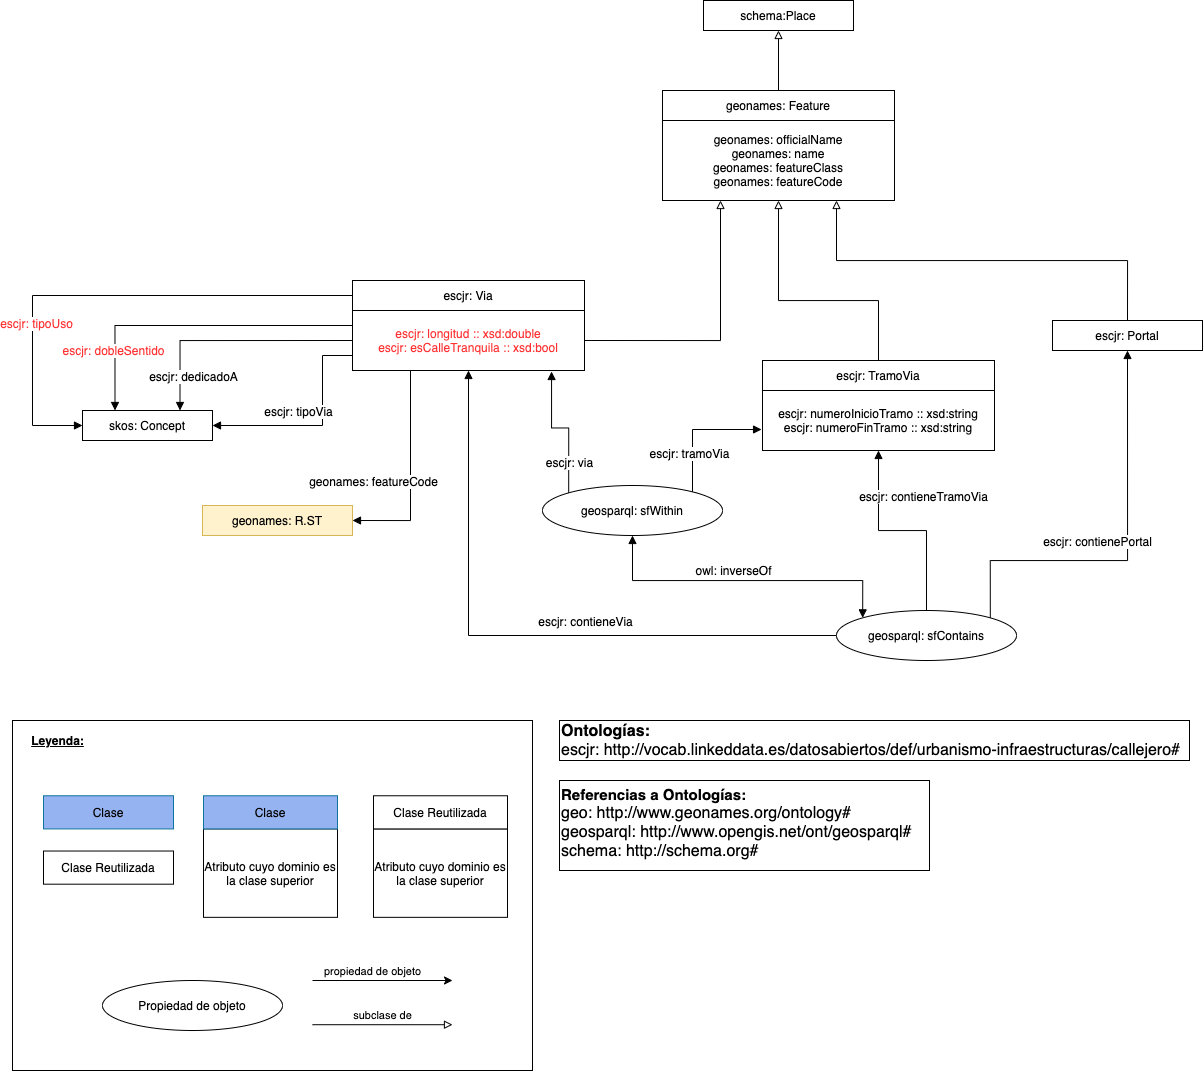
\includegraphics[angle=0, width=1\textwidth]{images/diagramaCallejero.png}  
	\caption{Diagrama de Ontología de Callejero}
	\label{fig:diagramaOntologCicloCarr}
\end{figure}


Se han añadadido las propiedades de objeto tipoUso y dobeSentido. La primera de ellas ha sido utilizada en los datasets de CicloCarriles y de CallesTranquilas y se refiere al uso dado (CicloCarril o Peatonal). La segunda únicamente en CallesTranquilas y como su nombre indica, representa el sentido único o doble de una calle.\newline
Se han añadido además dos propiedades de datos para la clase Via: longitud y esCalleTranquila. La primera se representa con un valor numérico decimal y formaba parte del dataset de Ciclocarriles y de CallesTranquilas. La segunda representa con un valor booleano si es o no una calle tranquila para ciclistas siguiendo el criterio del ayuntamiento.\newline
En las siguientes secciones se detallarán estas propiedades incluidas en la propuesta de modificación.


